% Added 18 October 2026. Append-only continuation for Day 1, 19 October 2026.
\begingroup
\date[19.10.2026]{19 October 2026}
\part[nopartpage]{From Green-Energy Ideas to a Shared Project}

\begin{frame}
\centering
\vfill
{\usebeamerfont{title}\color{fh-ooe-red}\Huge Two Months Later\ldots\par}
\vspace{.7em}
{\usebeamerfont{title}\color{fh-ooe-red}\Huge Ideas Have Evolved\par}
\vspace{1.5em}
{\Large You have developed your green-energy game.\par}
\vspace{.5em}
{\Large Your progress gives us a new perspective.\par}
\vfill
{\large From my first project ideas to \textbf{our shared design challenge}.\par}
\vfill
\end{frame}
\section[nosectionpage]{From Project Ideas to Your Game}
\begin{frame}{Four Ideas Within Our Shared Theme}{One Semester Focused on Green Energy}
When I prepared our three weeks together, I explored four ways to turn green energy into a practical IoT project.
\vspace{0.6em}
\begin{columns}[T,onlytextwidth]
\column{.24\textwidth}\centering
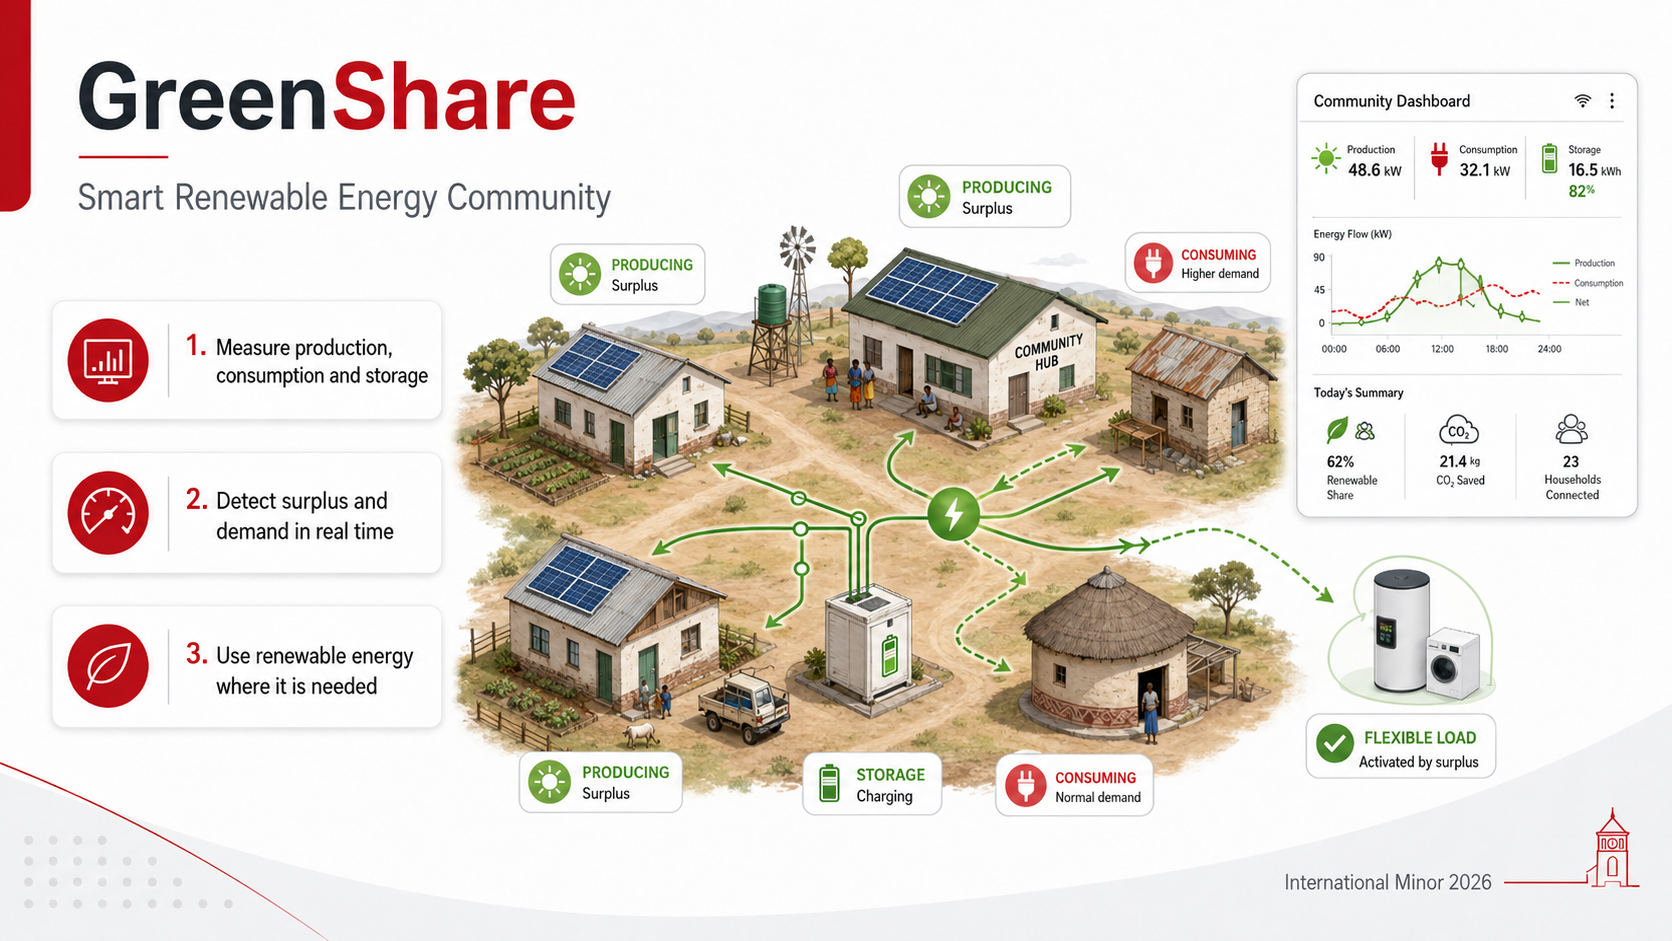
\includegraphics[width=\linewidth]{slides/035-ga-in-it-preintro/material/project-graphics/set-2/greenshare_renewable_energy_community.png}
\textbf{GreenShare}\\{\small Share energy}
\column{.24\textwidth}\centering
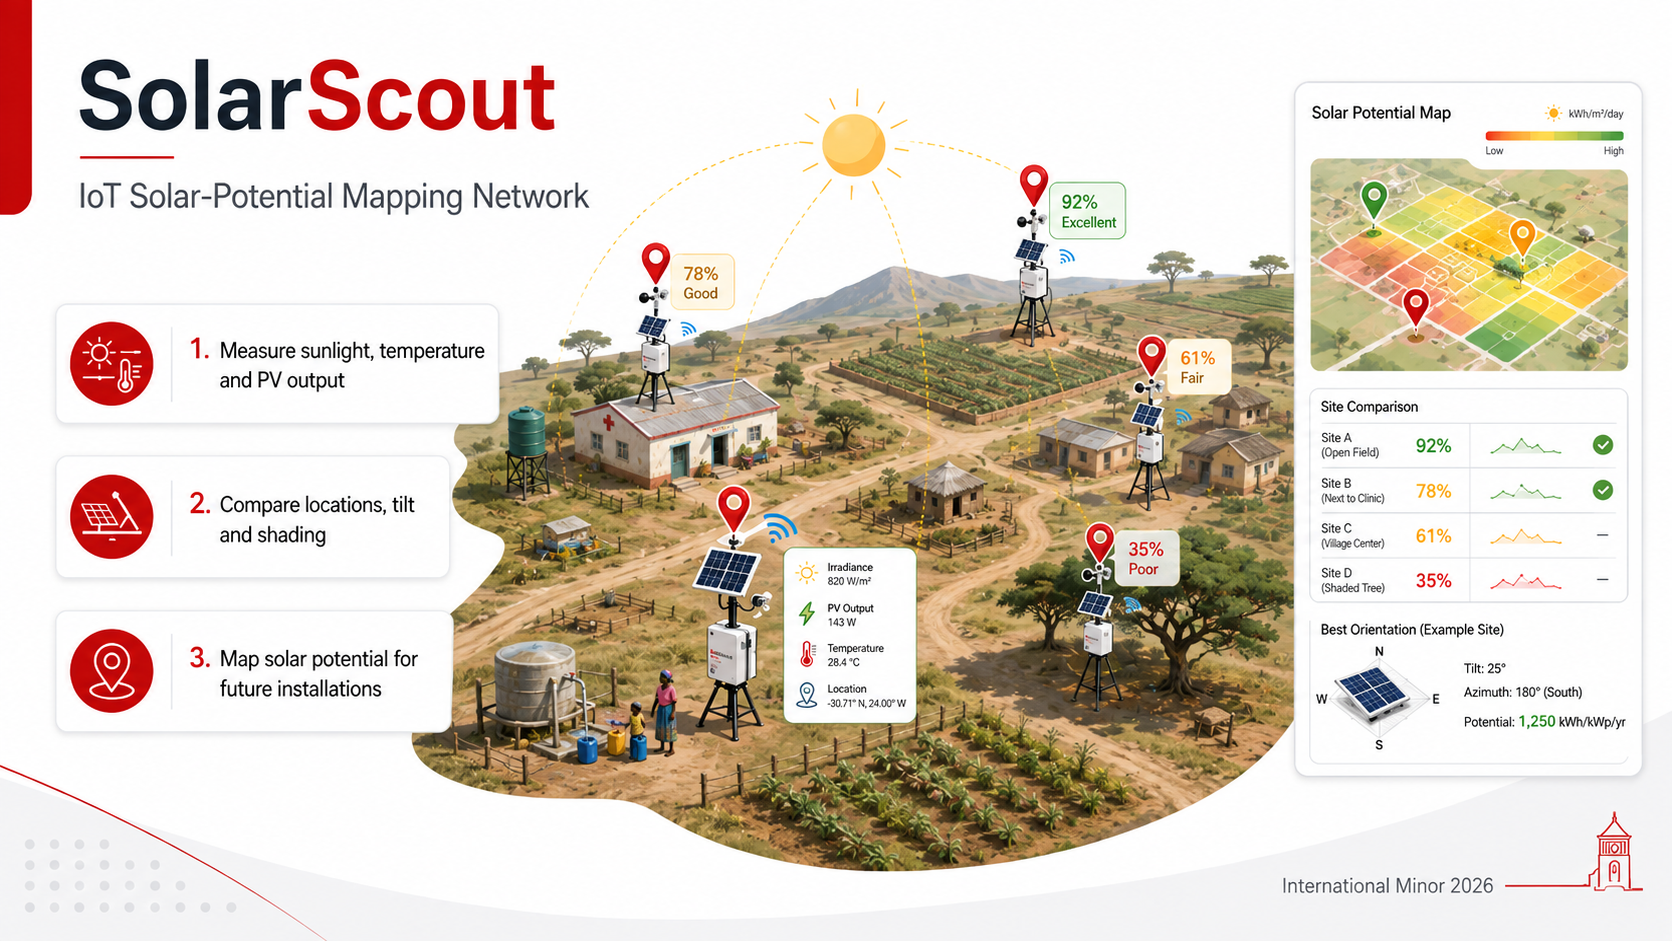
\includegraphics[width=\linewidth]{slides/035-ga-in-it-preintro/material/project-graphics/set-2/solarscout_mapping_solar_potential.png}
\textbf{SolarScout}\\{\small Understand generation}
\column{.24\textwidth}\centering
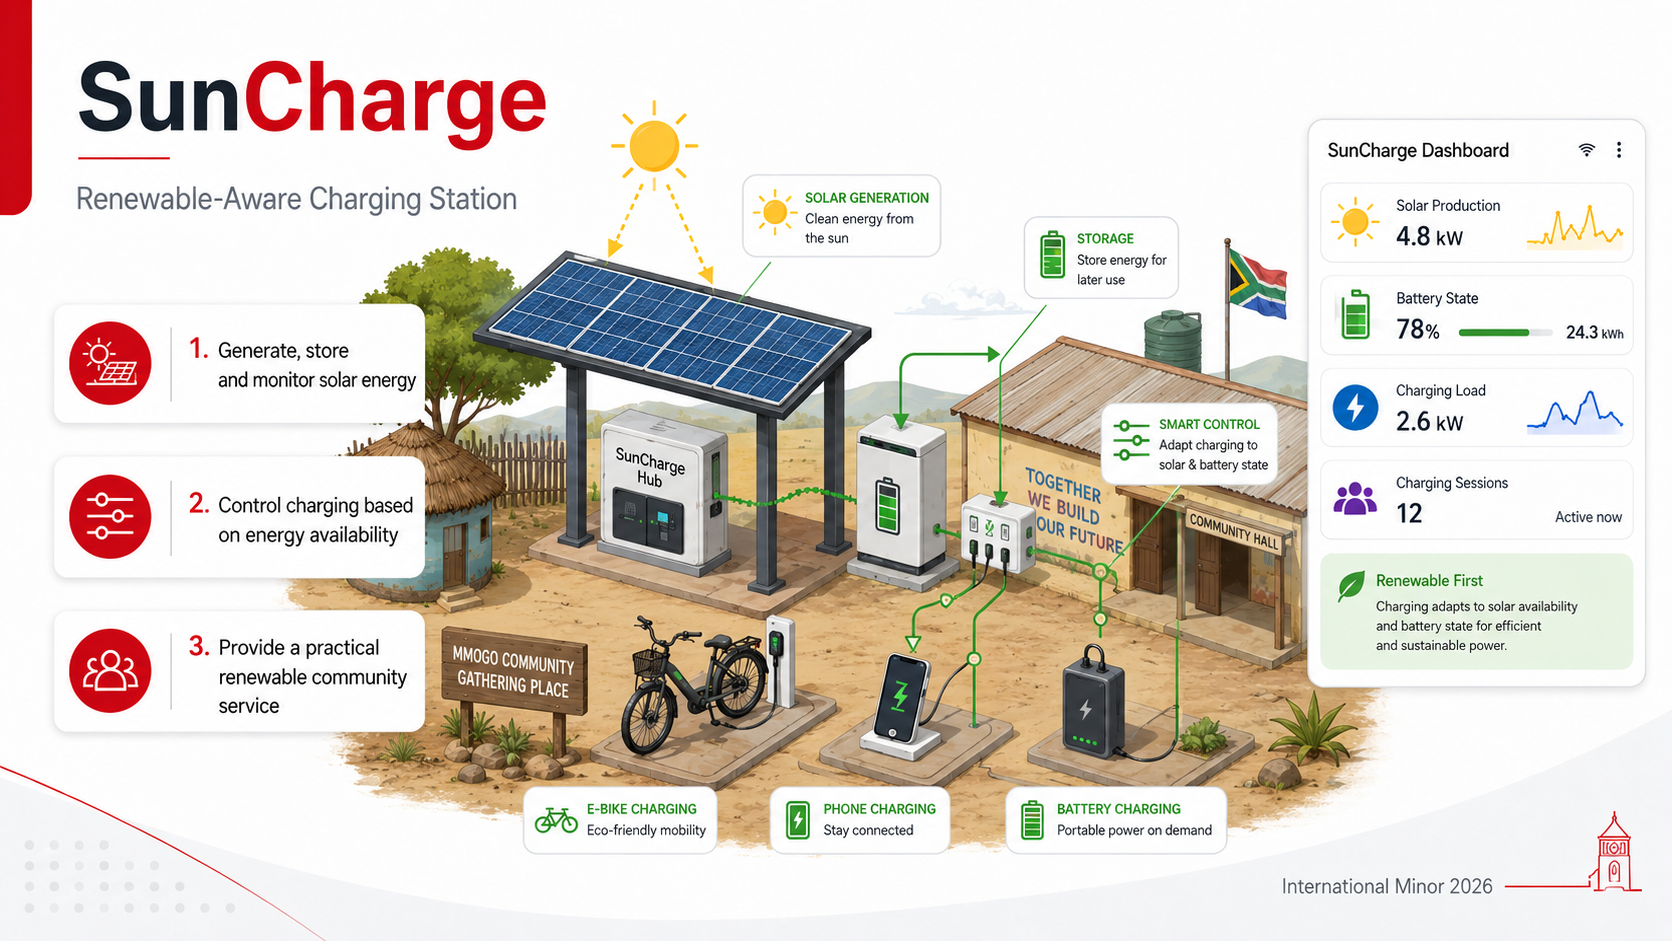
\includegraphics[width=\linewidth]{slides/035-ga-in-it-preintro/material/project-graphics/set-2/suncharge_community_renewable_charging_hub.png}
\textbf{SunCharge}\\{\small Store and supply energy}
\column{.24\textwidth}\centering
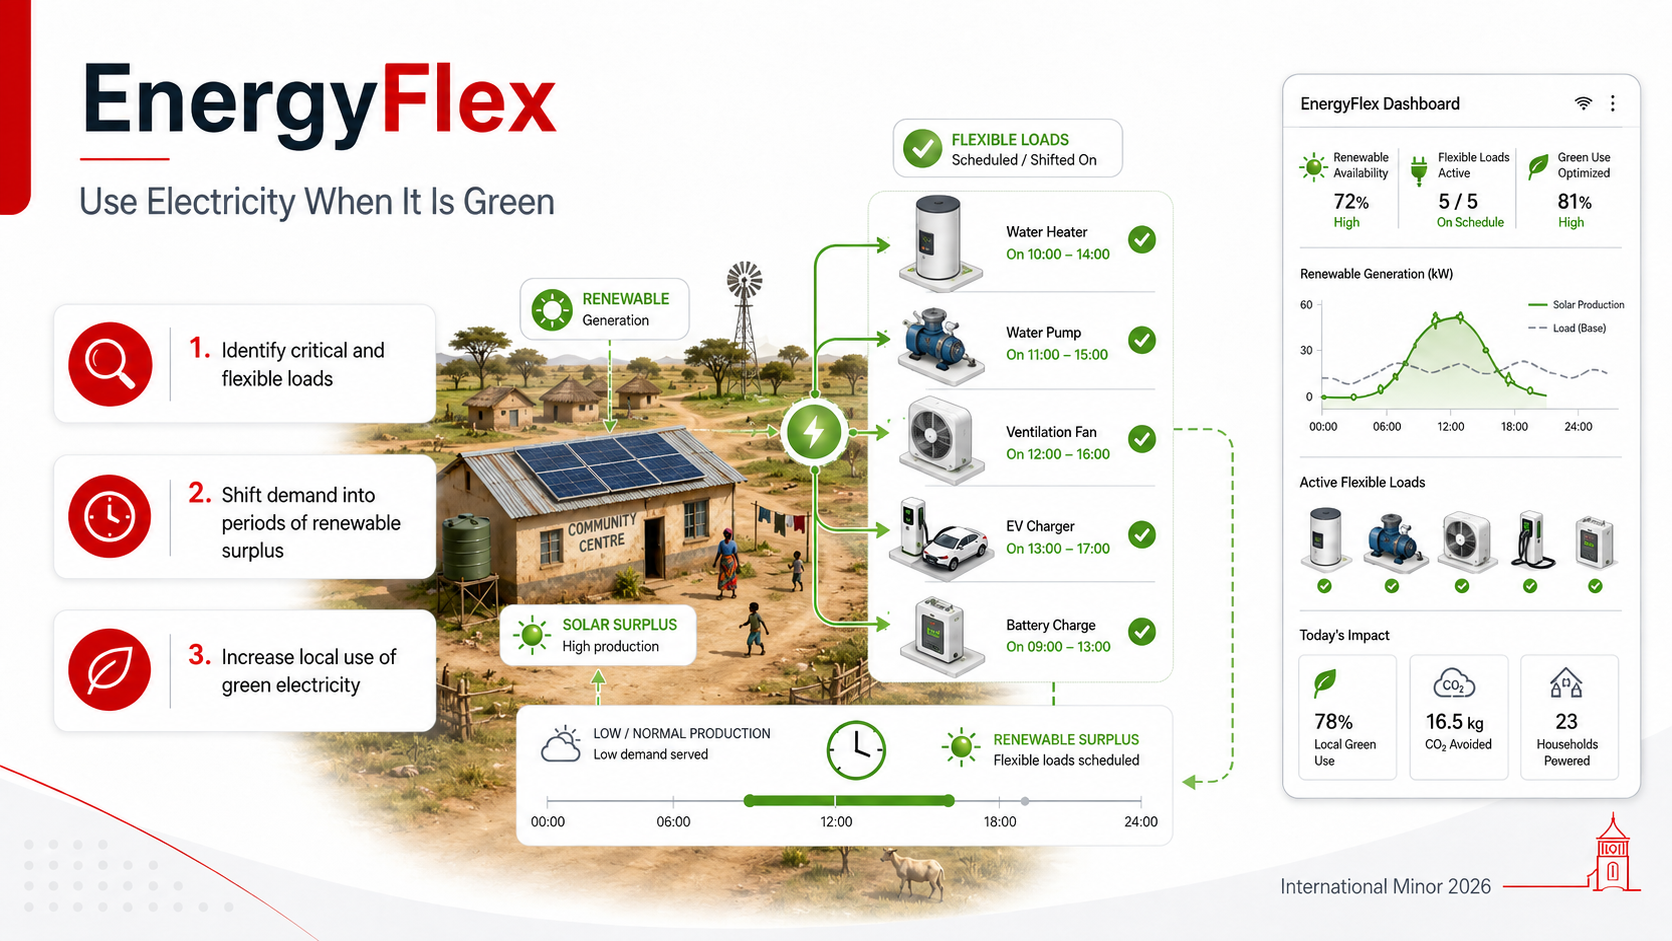
\includegraphics[width=\linewidth]{slides/035-ga-in-it-preintro/material/project-graphics/set-2/energyflex_renewable_village_dashboard.png}
\textbf{EnergyFlex}\\{\small Coordinate consumption}
\end{columns}
\begin{alertblock}{Ideas Develop When We Bring Them Together}
These were my initial starting points. Your green-energy game gives us an opportunity to develop them further.
\end{alertblock}
{\footnotesize Added 18 October 2026 \quad$\cdot$\quad Preparing for Day 1: 19 October 2026}
\end{frame}

\begin{frame}{Your Green-Energy Game Could Become Tangible}{A Physical Play Kit Connected to the Game You Are Developing}
You are already exploring green energy through a digital board game. Your project also includes physical gift packages for the communities you are addressing.
\begin{center}
\begin{tikzpicture}[every node/.style={align=center,font=\small}]
\node[draw=fh-ooe-red,fill=fh-ooe-red!6,rounded corners,text width=4.3cm,minimum height=1.4cm] (game) at (0,0) {\textbf{Your green-energy game}\\Players, choices, cooperation};
\node[draw=fh-ooe-red,fill=fh-ooe-red!6,rounded corners,text width=4.3cm,minimum height=1.4cm] (kit) at (7,0) {\textbf{A Smart Energy Play Kit}\\Real energy, devices, feedback};
\draw[<->,very thick,fh-ooe-red] (game) -- node[above]{Connected} (kit);
\end{tikzpicture}
\end{center}
During our three weeks, we could make these community-energy questions tangible in a small working kit, connected to your game and included in the gift package.
\begin{alertblock}{Our Shared Question}
What could players experience through real hardware that would enrich your game?
\end{alertblock}
\end{frame}

\begin{frame}{From Game Decisions to Physical Consequences}{Generate. Store. Consume. Share.}
A physical kit could make the energy relationships in your game visible and measurable.
\begin{center}
\begin{tikzpicture}[every node/.style={align=center,font=\small},box/.style={draw=fh-ooe-red,rounded corners,fill=fh-ooe-red!5,text width=4.6cm,minimum height=.8cm}]
\node[box] (a) at (0,0) {\textbf{Players make decisions}};
\node[box] (b) at (7,0) {\textbf{The physical system\\responds}};
\node[box] (c) at (7,-1.5) {\textbf{Measurements reveal\\consequences}};
\node[box] (d) at (0,-1.5) {\textbf{Players see the result\\in the game}};
\draw[->,thick,fh-ooe-red] (a)--(b);
\draw[->,thick,fh-ooe-red] (b)--(c);
\draw[->,thick,fh-ooe-red] (c)--(d);
\draw[->,thick,fh-ooe-red] (d)--(a);
\end{tikzpicture}
\end{center}
\begin{itemize}
\item Which game decisions should affect the kit?
\item Which measurements should influence the game?
\item What should players discover by experimenting?
\end{itemize}
\centering\alert{You define the relationship between gameplay and hardware.}
\end{frame}

\begin{frame}{Our Four Ideas Can Contribute to Your Kit}{Possible Building Blocks for One Shared Project}
\renewcommand{\arraystretch}{1.35}
\par\noindent\begin{tabularx}{\textwidth}{@{}l>{\raggedright\arraybackslash}X@{}}
\toprule
\textbf{Initial idea} & \textbf{Possible contribution}\\\midrule
GreenShare & Explore how players allocate or share limited energy.\\
SolarScout & Make renewable generation and changing conditions visible.\\
SunCharge & Explore storage, charging, and supplying consumers.\\
EnergyFlex & Connect priorities and timing to energy consumption.\\\bottomrule
\end{tabularx}\par
\begin{center}
\begin{tikzpicture}[every node/.style={font=\small,align=center}]
\node (a) at (0,0) {GreenShare};\node (b) at (3,0) {SolarScout};
\node (c) at (6,0) {SunCharge};\node (d) at (9,0) {EnergyFlex};
\node[draw=fh-ooe-red,rounded corners,fill=fh-ooe-red!6,minimum width=5cm] (kit) at (4.5,-1) {\textbf{Your shared kit design}};
\draw[->,fh-ooe-red] (a)--(kit);\draw[->,fh-ooe-red] (b)--(kit);
\draw[->,fh-ooe-red] (c)--(kit);\draw[->,fh-ooe-red] (d)--(kit);
\end{tikzpicture}
\end{center}
\small We might develop one idea, combine selected aspects, or reshape them around your game.\par
\alert{One coherent project for all eight students -- not four separate products.}
\end{frame}

\begin{frame}{The Challenge: Design a Self-Powered Play Kit}{A Direction from Me -- A Design from You}
My proposal: a small, real energy system powered by its own solar panel and battery, connected to your game.
\vspace{.5em}
\small\renewcommand{\arraystretch}{1.35}
\par\noindent\begin{tabularx}{\textwidth}{@{}>{\raggedright\arraybackslash}p{.40\textwidth}>{\raggedright\arraybackslash}X@{}}
\toprule
\textbf{Proposed direction} & \textbf{Decisions for you}\\\midrule
The kit supplies its own energy. & Under what conditions, and for how long?\\
Every included device uses that supply. & What is the complete energy budget?\\
A Raspberry Pi provides local administration and a dashboard. & What needs administration, visualization, and control?\\
Physical behaviour supports the game. & Which interactions are meaningful to players?\\
External power is optional. & How should development and demonstrations work?\\\bottomrule
\end{tabularx}\par
\begin{alertblock}{Your Design Responsibility}
You propose the first version, its architecture, and its success criteria.
\end{alertblock}
\end{frame}

\begin{frame}{We Have Many Possibilities}{Choose Equipment Because Your Design Needs It}
\begin{center}
\begin{tikzpicture}[every node/.style={align=center,font=\small},card/.style={draw=fh-ooe-red,rounded corners,fill=fh-ooe-red!5,text width=3.5cm,minimum height=1.1cm}]
\node[card] at (0,0) {\textbf{Microcontrollers}\\Embedded computation};
\node[card] at (4.4,0) {\textbf{Raspberry Pis}\\Local services};
\node[card] at (8.8,0) {\textbf{Beryl / GL.iNet routers}\\Local Wi-Fi networks};
\node[card] at (0,-1.5) {\textbf{LoRa and Bluetooth}\\Communication options};
\node[card] at (4.4,-1.5) {\textbf{Many different sensors}\\Observe the physical world};
\node[card] at (8.8,-1.5) {\textbf{Some actuators}\\Influence the physical world};
\end{tikzpicture}
\end{center}
\centering\textbf{Inspect $\longrightarrow$ Understand $\longrightarrow$ Experiment $\longrightarrow$ Choose}\par
\vspace{.7em}
\raggedright Check quantities, specifications, compatibility, condition, and energy consumption.
\begin{alertblock}{Available Options, Not Mandatory Ingredients}
Our inventory is the starting point. Your design determines what we need to buy.
\end{alertblock}
\end{frame}

\section[nosectionpage]{One Team, One System}
\begin{frame}{One Project. Eight Students. Four Pairs.}{A Proposed Division of Responsibilities}
\small\renewcommand{\arraystretch}{1.35}
\par\noindent\begin{tabularx}{\textwidth}{@{}>{\raggedright\arraybackslash}p{.21\textwidth}>{\raggedright\arraybackslash}X >{\raggedright\arraybackslash}p{.26\textwidth}@{}}
\toprule
\textbf{Pair} & \textbf{Responsibility} & \textbf{Central question}\\\midrule
\textbf{Energy and power} & Generation, storage, distribution, protection, and the whole-kit energy budget. & How will the kit power itself?\\
\textbf{Devices and measurement} & Sensors, consumers, actuators, and MCU software. & What must we measure and influence?\\
\textbf{Infrastructure and dashboard} & Networking, Raspberry Pi services, device administration, and visualization. & How will the system communicate and become understandable?\\
\textbf{Game and kit experience} & Game interaction, player experience, packaging, and instructions. & How does the kit support the game and its users?\\\bottomrule
\end{tabularx}\par
\vspace{.6em}
\alert{Agree the responsibilities together. Each pair leads an area; all eight own the result.}
\end{frame}

\begin{frame}{The Interfaces Are Shared Work}{Four Areas Must Become One Working System}
\begin{center}
\begin{tikzpicture}[every node/.style={align=center,font=\small},box/.style={draw=fh-ooe-red,rounded corners,fill=fh-ooe-red!5,text width=3.3cm,minimum height=.7cm}]
\node[box] (a) at (0,0) {\textbf{Energy and power}\\{\scriptsize Power requirements}};
\node[box] (b) at (8,0) {\textbf{Devices and measurement}\\{\scriptsize Measurements / commands}};
\node[box] (c) at (0,-2.8) {\textbf{Infrastructure and dashboard}\\{\scriptsize User interaction}};
\node[box] (d) at (8,-2.8) {\textbf{Game and kit experience}\\{\scriptsize Game events}};
\node[draw=fh-ooe-red,fill=fh-ooe-red!15,rounded corners,text width=3.4cm,minimum height=.9cm] (core) at (4,-1.4) {\textbf{Our shared\\system design}};
\draw[<->,fh-ooe-red] (a)--(core);
\draw[<->,fh-ooe-red] (b)--(core);
\draw[<->,fh-ooe-red] (c)--(core);
\draw[<->,fh-ooe-red] (d)--(core);
\end{tikzpicture}
\end{center}
\small What does your subsystem \textbf{need}? What does it \textbf{provide}? How will you \textbf{demonstrate the connection}?\par
\vspace{.5em}
\alert{Agree early. Record decisions. Integrate frequently.}\par
\footnotesize Include the Raspberry Pi, router, and idle devices in the energy budget.
\end{frame}

\section[nosectionpage]{Our Three Weeks}
\begin{frame}{Our Three Weeks}{From Your Design to a Demonstrated Result}
\begin{center}
\begin{tikzpicture}[every node/.style={font=\small,align=center}]
\draw[->,very thick,fh-ooe-red] (0,0)--(11,0);
\foreach \x/\label in {1/Explore and decide,5.3/Build and connect,9.5/Test and refine}{\fill[fh-ooe-red] (\x,0) circle (3pt);\node[above] at (\x,.15) {\label};}
\node[below] at (5.5,-.1) {\textbf{Integration throughout}};
\end{tikzpicture}
\end{center}
\small\renewcommand{\arraystretch}{1.3}
\par\noindent\begin{tabularx}{\textwidth}{@{}l>{\raggedright\arraybackslash}X>{\raggedright\arraybackslash}X@{}}
\toprule
\textbf{Week} & \textbf{Focus} & \textbf{Evidence of progress}\\\midrule
\textbf{1} & Understand the game, inspect equipment, define the first version, investigate uncertainties, order missing parts. & A justified design, purchasing decisions, and early experiments.\\
\textbf{2} & Develop the agreed functions and integrate the subsystems. & Working interactions across the system.\\
\textbf{3} & Evaluate requirements; improve reliability, usability, packaging, and documentation. & A demonstrable kit with clearly explained capabilities and limitations.\\\bottomrule
\end{tabularx}\par
\vspace{.5em}\alert{Additional features depend on progress toward your agreed first version.}
\end{frame}

\section[nosectionpage]{Day 1: Design and Planning}
\begin{frame}{Day 1 -- Understand Before Choosing}{Monday, 19 October 2026 -- Morning}
\small\renewcommand{\arraystretch}{1.35}
\par\noindent\begin{tabularx}{\textwidth}{@{}l>{\raggedright\arraybackslash}X >{\raggedright\arraybackslash}p{.30\textwidth}@{}}
\toprule
\textbf{Time} & \textbf{Activity} & \textbf{Intended result}\\\midrule
08:50--09:20 & Introduction, project context, and your game & Shared understanding\\
09:20--10:00 & Discuss meaningful game--kit connections & Candidate interactions and questions\\
10:00--10:15 & \textit{Break} & \\
10:15--11:00 & Explore and inventory equipment & Resources and uncertainties\\
11:00--11:45 & Discuss requirements and possible system designs & A proposed direction\\
11:45--12:15 & Agree responsibilities and investigation tasks & Four pairs ready for the afternoon\\
12:15--13:00 & \textit{Lunch} & \\\bottomrule
\end{tabularx}\par
\vspace{.6em}
\footnotesize The introductory presentation and original project proposals are part of this morning programme.\par
\alert{Working schedule -- adjust discussion time to what we discover.}
\end{frame}

\begin{frame}{Day 1 -- Turn Ideas into Decisions}{Monday, 19 October 2026 -- Afternoon}
\small\renewcommand{\arraystretch}{1.45}
\par\noindent\begin{tabularx}{\textwidth}{@{}l>{\raggedright\arraybackslash}X >{\raggedright\arraybackslash}p{.30\textwidth}@{}}
\toprule
\textbf{Time} & \textbf{Activity} & \textbf{Intended result}\\\midrule
13:00--14:00 & Investigate in pairs: inspect specifications, measure, experiment, compare options & Evidence supporting design choices\\
14:00--14:15 & \textit{Break} & \\
14:15--15:00 & Combine proposals and resolve interface conflicts & One coherent first-version design\\
15:00--15:35 & Review missing equipment and purchasing priorities & A justified equipment list\\
15:35--16:00 & Present the proposal and agree next steps & Shared decisions, owners, immediate tasks\\\bottomrule
\end{tabularx}\par
\begin{alertblock}{Evidence Before Purchases}
A useful experiment can prevent an unnecessary purchase -- or reveal a missing requirement.
\end{alertblock}
\end{frame}

\begin{frame}{By 16:00: Your First-Version Proposal}{The First Version Should Exist as a Complete, Agreed Design}
\small\renewcommand{\arraystretch}{1.25}
\par\noindent\begin{tabularx}{\textwidth}{@{}>{\raggedright\arraybackslash}p{.25\textwidth}>{\raggedright\arraybackslash}X@{}}
\toprule
\textbf{Deliverable} & \textbf{What you should be able to explain}\\\midrule
\textbf{Game connection} & Who the kit serves and how it supports your game.\\
\textbf{Scope and success criteria} & What you will build, what you defer, and how you will evaluate it.\\
\textbf{System diagram} & Components, power paths, communication, and interfaces.\\
\textbf{Energy assumptions} & Operating conditions and duration; estimates and measurements still needed.\\
\textbf{\color{fh-ooe-red}Equipment list} & What we have, what we must buy, and why.\\
\textbf{Work plan} & Responsibilities, dependencies, uncertainties, and next steps.\\\bottomrule
\end{tabularx}\par
\vspace{.5em}
\footnotesize Purchasing list: item, required / available quantities, specification, purpose, cost, delivery time, priority.\par
\vspace{.5em}
\normalsize\alert{A design you can explain. Choices you can justify. A shopping list we can act on.}
\end{frame}
\endgroup
